%% chapter13_slides.tex
%% Chapter 13: Conclusions and Future Developments
%% Nature Inspired Optimisation for Delivery Problems (2022)
%% Self-contained lecture slides -- no presenter required.
%%
%% Compile twice:
%%   pdflatex -interaction=nonstopmode chapter13_slides.tex
%%   pdflatex -interaction=nonstopmode chapter13_slides.tex

\documentclass[aspectratio=169,10pt]{beamer}

\usetheme{Madrid}
\usecolortheme{seahorse}

%% ---- packages ----
\usepackage[T1]{fontenc}
\usepackage[utf8]{inputenc}
\usepackage{lmodern}
\usepackage{amsmath,amssymb}
\usepackage{graphicx}
\usepackage{booktabs}
\usepackage{listings}
\usepackage{xcolor}
\usepackage{tikz}
\usepackage{pgfplots}
\pgfplotsset{compat=1.18}
\usepackage{url}
\usepackage{hyperref}
\usepackage{array}
\usepackage{microtype}

\graphicspath{{figures/}}

%% ---- listings style ----
\lstset{
  language=Python,
  basicstyle=\ttfamily\scriptsize,
  numbers=left,
  numberstyle=\tiny\color{gray},
  frame=single,
  backgroundcolor=\color{gray!7},
  commentstyle=\color{green!50!black}\itshape,
  keywordstyle=\color{blue!70!black}\bfseries,
  stringstyle=\color{orange!80!black},
  showstringspaces=false,
  breaklines=true,
  tabsize=4,
}

%% ---- footer ----
\setbeamertemplate{footline}[frame number]
\setbeamertemplate{navigation symbols}{}

%% ---- title info ----
\title[Ch.~13 Conclusions]{Chapter 13: Conclusions and Future Developments}
\subtitle{Nature Inspired Optimisation for Delivery Problems (2022)}
\author{Based on: T.~Cherrett, J.~Holguin-Veras \textit{et al.}}
\date{2022 --- Slides prepared for self-study}

%% ===================================================================
\begin{document}
%% ===================================================================

%% ---- Title ----
\begin{frame}
  \titlepage
\end{frame}

%% ---- Table of Contents ----
\begin{frame}[allowframebreaks]{Chapter 13 --- Overview}

  This final chapter of the book takes stock of everything covered in the
  preceding twelve chapters and looks ahead to three major areas where the
  field of delivery optimisation is expected to evolve rapidly.

  \bigskip
  \begin{block}{Chapter Structure}
    \begin{itemize}
      \item \textbf{Section 13.1 --- Software, Algorithms and AI.}
            How the next generation of optimisation \emph{software} will be
            designed, focusing on the concept of a \emph{domain-specific AI
            solver} that can autonomously understand and solve a broad class
            of delivery problems.
      \item \textbf{Section 13.2 --- Developments in Transportation.}
            Emerging physical technologies --- autonomous vehicles, drones,
            electric fleets, and the use of public transport as a freight
            carrier --- that will reshape the landscape in which
            optimisation algorithms must operate.
      \item \textbf{Section 13.3 --- Consumers.}
            How changing consumer expectations (speed, sustainability,
            transparency) and growing awareness of climate change are
            creating new requirements for delivery systems.
    \end{itemize}
  \end{block}

  \bigskip
  \begin{alertblock}{Why This Chapter Matters}
    Throughout this book, the authors have shown that nature-inspired
    algorithms (evolutionary algorithms, ant-colony optimisation,
    particle-swarm optimisation, etc.) can solve difficult routing problems.
    This concluding chapter asks: \emph{where does the field go from here?}
    The answer lies at the intersection of better AI, better physical
    transport technology, and better understanding of what consumers
    actually want.
  \end{alertblock}

\end{frame}

%% ====================================================================
\section{13.1 Software, Algorithms and AI}
%% ====================================================================

\begin{frame}[allowframebreaks]{13.1 Software, Algorithms and AI --- The Challenge}

  One of the most practically important questions in delivery logistics
  is deceptively simple: \emph{how should a company choose the right
  optimisation software for their specific problem?}

  \bigskip
  The difficulty is that real delivery problems come in an enormous
  variety of forms.  A parcel carrier faces a very different problem
  from a food-delivery platform or a humanitarian aid organisation,
  yet all of them share a common structure: vehicles, customers, routes,
  and objectives such as cost or time.

  \bigskip
  \begin{block}{Three Existing Strategies --- and Their Weaknesses}
    The book identifies three strategies currently used to match problems
    to solvers, and explains why none of them is fully satisfactory:

    \medskip
    \begin{enumerate}
      \item \textbf{Build a custom solver for each variant.}
            This produces the best possible solution quality for a given
            problem, but the cost is enormous: a specialist team must be
            assembled for every new variant (time windows, multiple depots,
            heterogeneous fleets, etc.), and the resulting code is rarely
            reusable.

      \item \textbf{Build one enormous universal solver.}
            Such a solver would cover all variants in a single codebase.
            While technically conceivable, the result is an unwieldy,
            hard-to-maintain system that is difficult for practitioners
            to understand and configure correctly.

      \item \textbf{Force the problem to fit an existing solver.}
            This is the most common approach in practice: simplify or
            distort the real problem so that an off-the-shelf package
            can handle it.  The cost is solution quality --- the algorithm
            optimises the \emph{wrong} objective or ignores important
            constraints.
    \end{enumerate}
  \end{block}

  \bigskip
  \begin{center}
    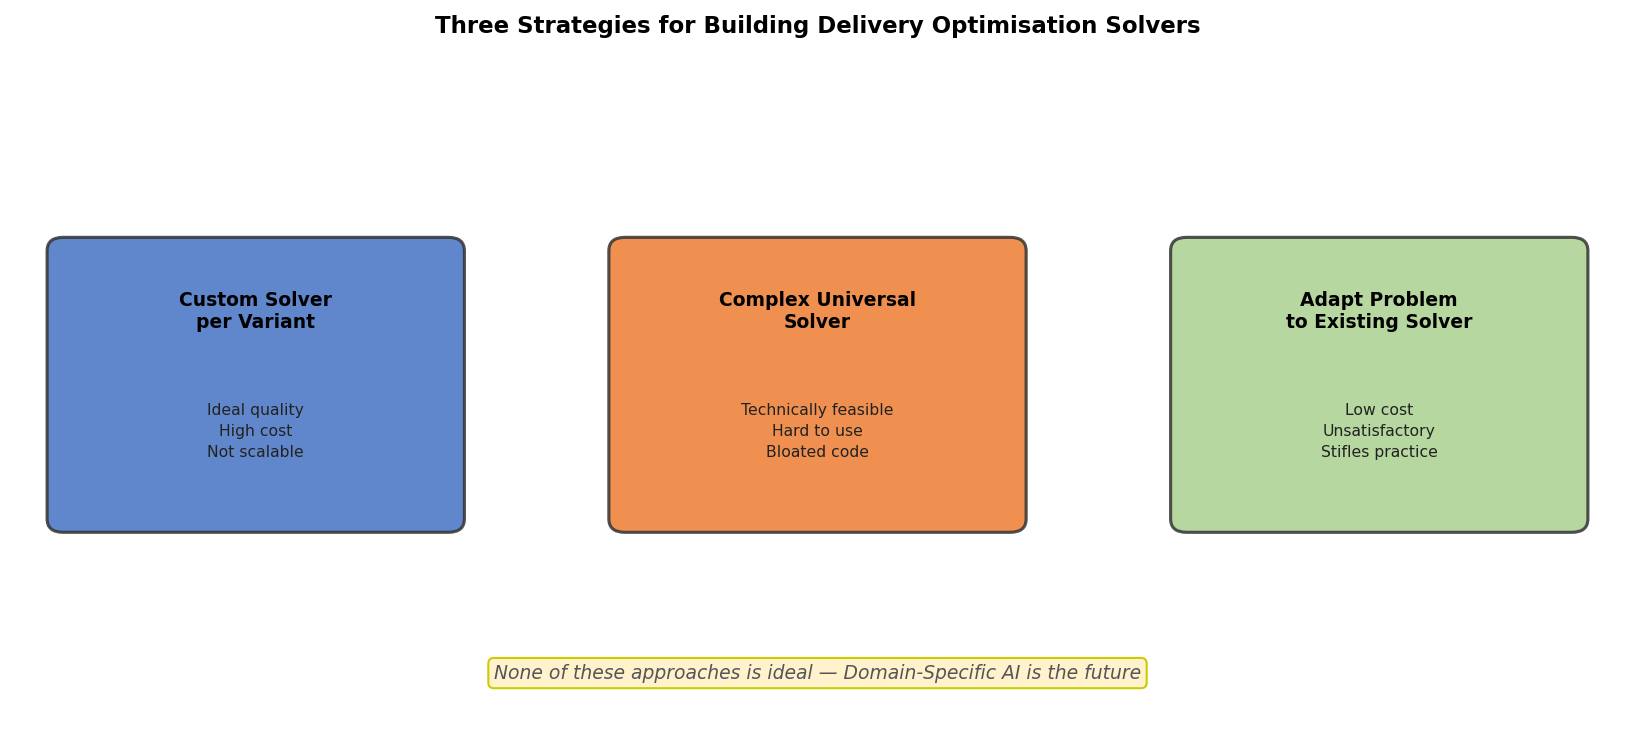
\includegraphics[width=0.85\textwidth]{software_strategies.png}
  \end{center}

  \begin{alertblock}{Key Insight}
    All three strategies represent a compromise.  The ideal solution
    would be software that \emph{understands} the problem
    deeply --- much as a human expert does --- and constructs the
    right algorithm automatically.  This is the vision for the next
    generation of AI-driven optimisation tools.
  \end{alertblock}

\end{frame}

%% ---- Adaptive Solver ----
\begin{frame}[allowframebreaks]{13.1 The Vision: An Adaptive Problem Solver}

  The book proposes a more ambitious goal: building an
  \textbf{adaptive problem solver} that sits somewhere between
  a rigid specialist tool and the far-future concept of
  Artificial General Intelligence (AGI).

  \bigskip
  The key idea is that the solver should be able to do the following
  things automatically, without requiring manual reconfiguration
  for each new problem instance:

  \bigskip
  \begin{block}{Capabilities of an Adaptive Solver}
    \begin{itemize}
      \item \textbf{Understand the problem from a description.}
            Given a plain-language or structured description of a new
            delivery scenario, the solver recognises which class of
            problem it belongs to (TSP-like? capacitated VRP?
            time-windowed? multi-depot?).

      \item \textbf{Select and configure appropriate algorithms.}
            Rather than applying a fixed metaheuristic, the solver
            draws on a library of algorithmic building blocks
            --- local-search operators, crossover strategies,
            population-management schemes --- and assembles the
            combination most likely to perform well for this problem class.

      \item \textbf{Learn from experience.}
            Machine learning techniques allow the solver to track
            which algorithm configurations have worked well on
            similar problems in the past, and to give preference to
            those configurations when encountering new but structurally
            similar instances.

      \item \textbf{Present a diverse set of solutions.}
            Using an \emph{illumination} approach (such as MAP-Elites,
            covered in Chapter 6), the solver maintains a rich archive
            of solutions that trade off different objectives
            (e.g., cost vs.\ carbon emissions vs.\ delivery time),
            so that decision-makers can explore the trade-off space.
    \end{itemize}
  \end{block}

  \bigskip
  \begin{center}
    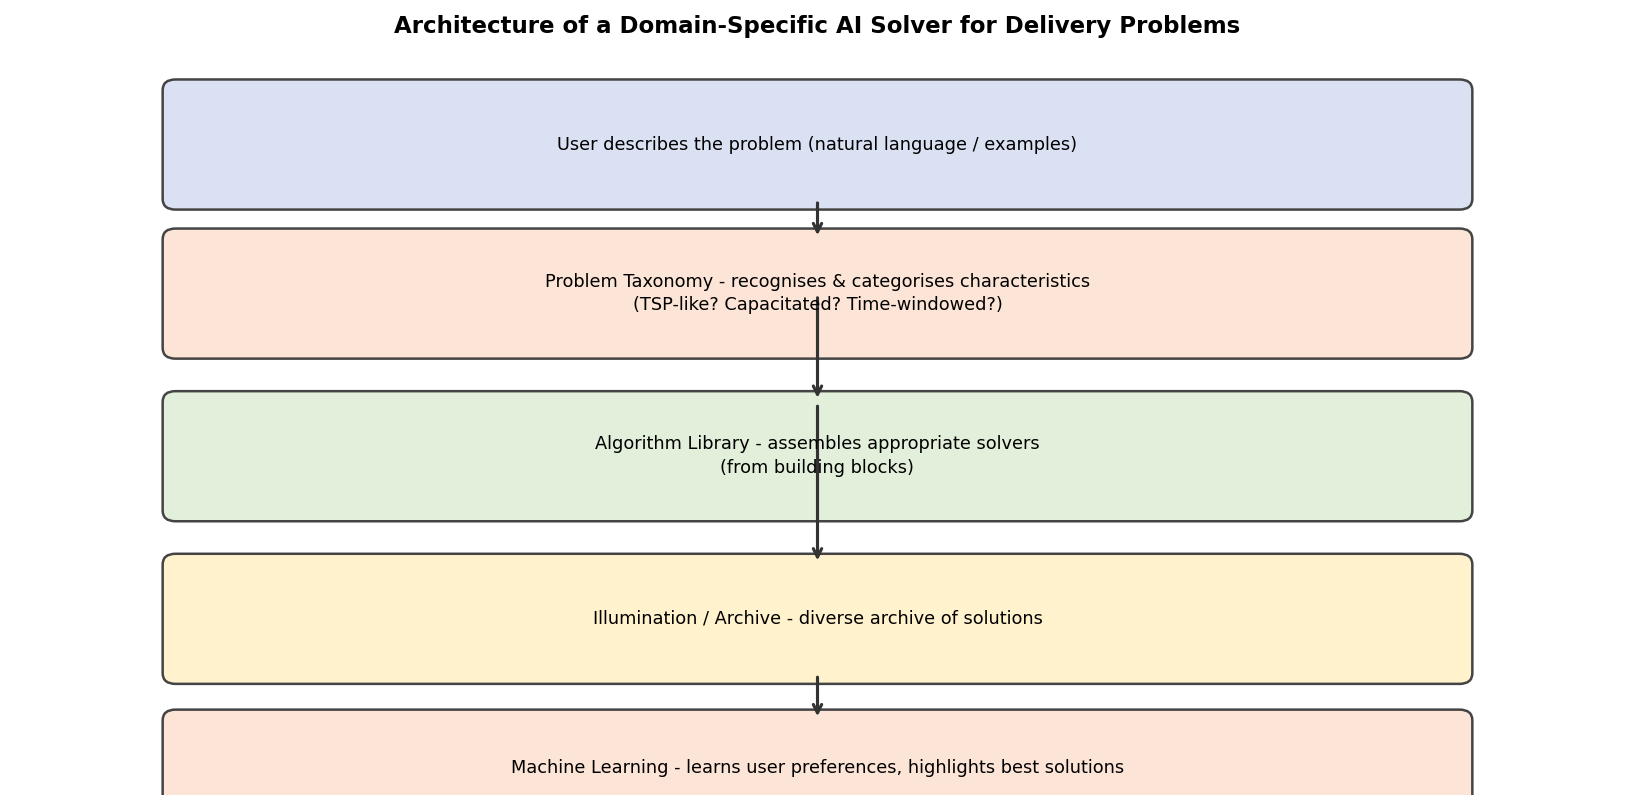
\includegraphics[width=0.82\textwidth]{domain_specific_ai.png}
  \end{center}

  \begin{alertblock}{How to Read This Diagram}
    The architecture flows \emph{downward}.  A user provides a
    problem description at the top; the taxonomy layer classifies
    it; the algorithm library assembles a solver; the illumination
    layer generates a diverse solution archive; and the machine-learning
    layer surfaces the solutions that best match the user's implicit
    preferences (for example, preferring greener routes even if the
    user has not explicitly requested this).
  \end{alertblock}

\end{frame}

%% ---- AGI Timeline ----
\begin{frame}[allowframebreaks]{13.1 The Road to AGI --- A Broader Perspective}

  The adaptive solver described above is a near-term, \emph{domain-specific}
  AI system: it is highly capable within delivery logistics, but it is
  not a general-purpose reasoner.  The book situates this in a longer
  trajectory:

  \bigskip
  \begin{center}
    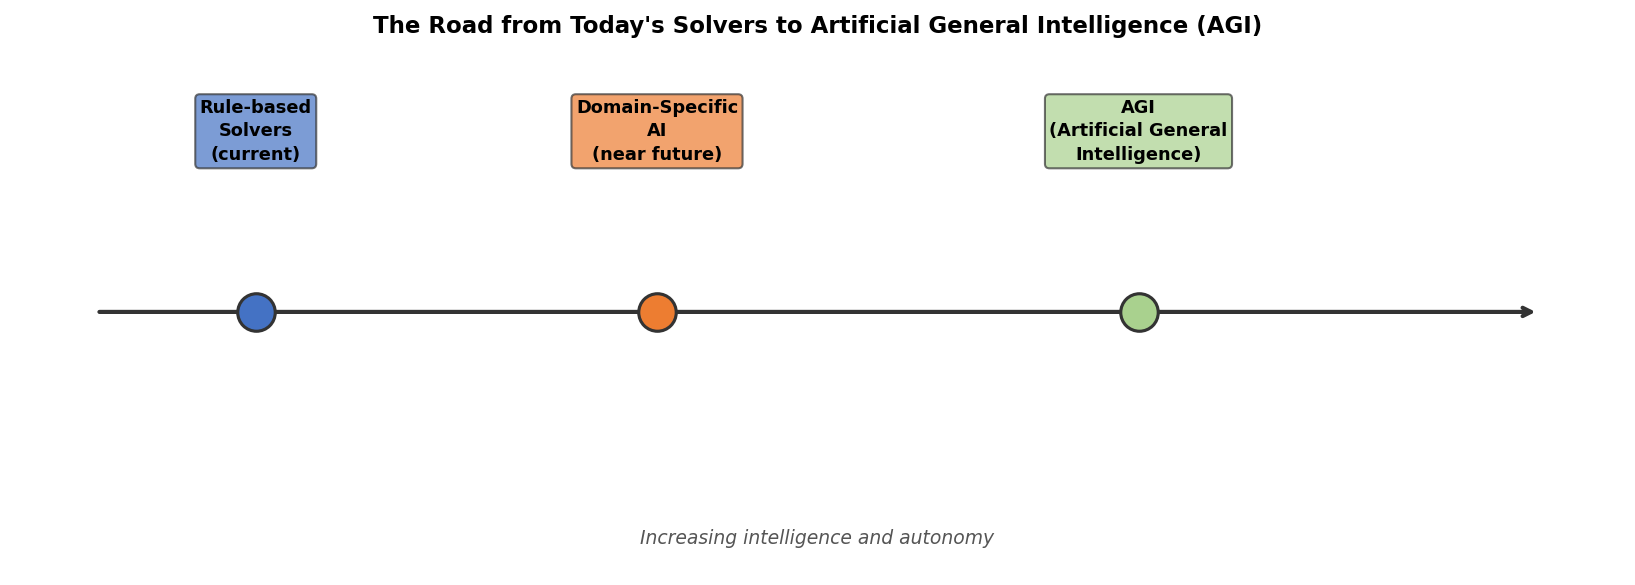
\includegraphics[width=0.82\textwidth]{ai_evolution.png}
  \end{center}

  \bigskip
  \begin{block}{Three Stages in the Evolution of AI for Logistics}
    \begin{description}
      \item[Rule-based solvers (today).]
        Current commercial software applies a fixed set of rules and
        a single metaheuristic.  The user must manually select the
        algorithm and tune its parameters.  Solutions are good but the
        system has no understanding of the problem --- it simply
        executes a procedure.

      \item[Domain-specific AI (near future).]
        Software that understands problem structure, assembles algorithms
        automatically, and learns from previous runs.  This is the
        target described in Section 13.1.

      \item[Artificial General Intelligence (AGI).]
        A system with human-level reasoning across arbitrary domains.
        AGI could, in principle, solve \emph{any} combinatorial
        optimisation problem after reading a description.
        Futurist Ray Kurzweil (cited in the book) argued that
        human-level AI could arrive as early as 2029, though this
        remains a subject of active debate.
    \end{description}
  \end{block}

  \bigskip
  \begin{alertblock}{Practical Takeaway}
    Whether or not AGI arrives by 2029, the authors argue that
    \emph{the development of domain-specific AI solvers for
    logistics is already underway and will fundamentally change
    how companies deploy optimisation software.}
    The techniques in this book --- illumination, multi-objective
    search, real-world data integration --- are the building blocks
    of that future.
  \end{alertblock}

\end{frame}

%% ---- Python: Intelligent Solver Skeleton ----
\begin{frame}[fragile]{Python: Skeleton of an Adaptive Solver}

  The following Python sketch illustrates how an adaptive solver
  might be structured in practice.  The core idea is that the
  \texttt{solve()} function does not hard-code a specific algorithm;
  instead it \emph{selects} the best available algorithm based on
  the problem's characteristics.

  \smallskip
  \begin{lstlisting}
class AdaptiveSolver:
    """
    Domain-specific AI solver for delivery problems.
    Automatically selects and configures the best algorithm
    based on problem characteristics detected at runtime.
    """

    def __init__(self, algorithm_library):
        # algorithm_library is a dict: name -> algorithm class
        self.library = algorithm_library
        self.performance_log = {}   # tracks past performance

    def classify_problem(self, problem):
        """
        Inspect the problem and return a dict of characteristics.
        E.g.: {'type': 'CVRP', 'n_customers': 200,
               'has_time_windows': True, 'multi_depot': False}
        """
        characteristics = {}
        characteristics['n_customers'] = len(problem.customers)
        characteristics['has_time_windows'] = problem.time_windows is not None
        characteristics['has_capacity']     = problem.vehicle_capacity is not None
        characteristics['multi_depot']      = len(problem.depots) > 1
        # Classify overall type
        if characteristics['has_time_windows']:
            characteristics['type'] = 'VRPTW'
        elif characteristics['has_capacity']:
            characteristics['type'] = 'CVRP'
        else:
            characteristics['type'] = 'TSP'
        return characteristics

    def select_algorithm(self, characteristics):
        """
        Choose the best algorithm for the detected problem type.
        Uses past performance data if available.
        """
        problem_type = characteristics['type']
        n = characteristics['n_customers']

        # Default rules based on problem size and type
        if n < 50:
            preferred = 'exact_branch_and_bound'
        elif problem_type == 'VRPTW':
            preferred = 'ant_colony_optimisation'
        elif problem_type == 'CVRP' and n < 500:
            preferred = 'evolutionary_algorithm'
        else:
            preferred = 'simulated_annealing'

        # Override with learned preference if data exists
        key = (problem_type, n // 100)   # coarse bucket
        if key in self.performance_log:
            best_seen = min(self.performance_log[key],
                            key=lambda x: x['cost'])
            preferred = best_seen['algorithm']

        return self.library.get(preferred, self.library['evolutionary_algorithm'])

    def solve(self, problem, time_limit=60):
        """
        Main entry point. Returns the best solution found.
        """
        characteristics = self.classify_problem(problem)
        AlgorithmClass  = self.select_algorithm(characteristics)
        algorithm = AlgorithmClass(time_limit=time_limit)

        solution = algorithm.run(problem)

        # Log performance for future learning
        key = (characteristics['type'], characteristics['n_customers'] // 100)
        self.performance_log.setdefault(key, []).append({
            'algorithm': AlgorithmClass.__name__,
            'cost': solution.total_cost,
        })
        return solution
  \end{lstlisting}

  \smallskip
  \textbf{Line-by-line explanation:}
  \begin{itemize}
    \item Lines 14--21: \texttt{classify\_problem} inspects the
          problem object and fills a dictionary with structural
          characteristics.  This is the ``taxonomy'' step.
    \item Lines 23--42: \texttt{select\_algorithm} applies
          default rules (smaller problems use exact methods;
          larger ones use metaheuristics) and then \emph{overrides}
          those defaults with learned preferences from past runs.
    \item Lines 44--55: \texttt{solve} ties everything together:
          classify, select, run, and log the result for future use.
  \end{itemize}

\end{frame}

%% ====================================================================
\section{13.2 Developments in Transportation}
%% ====================================================================

\begin{frame}[allowframebreaks]{13.2 Developments in Transportation --- Overview}

  Even the most sophisticated algorithm can only work with the
  physical transport infrastructure available to it.  Section 13.2
  examines how the physical side of delivery is changing, and why
  these changes create new and harder optimisation problems.

  \bigskip
  \begin{center}
    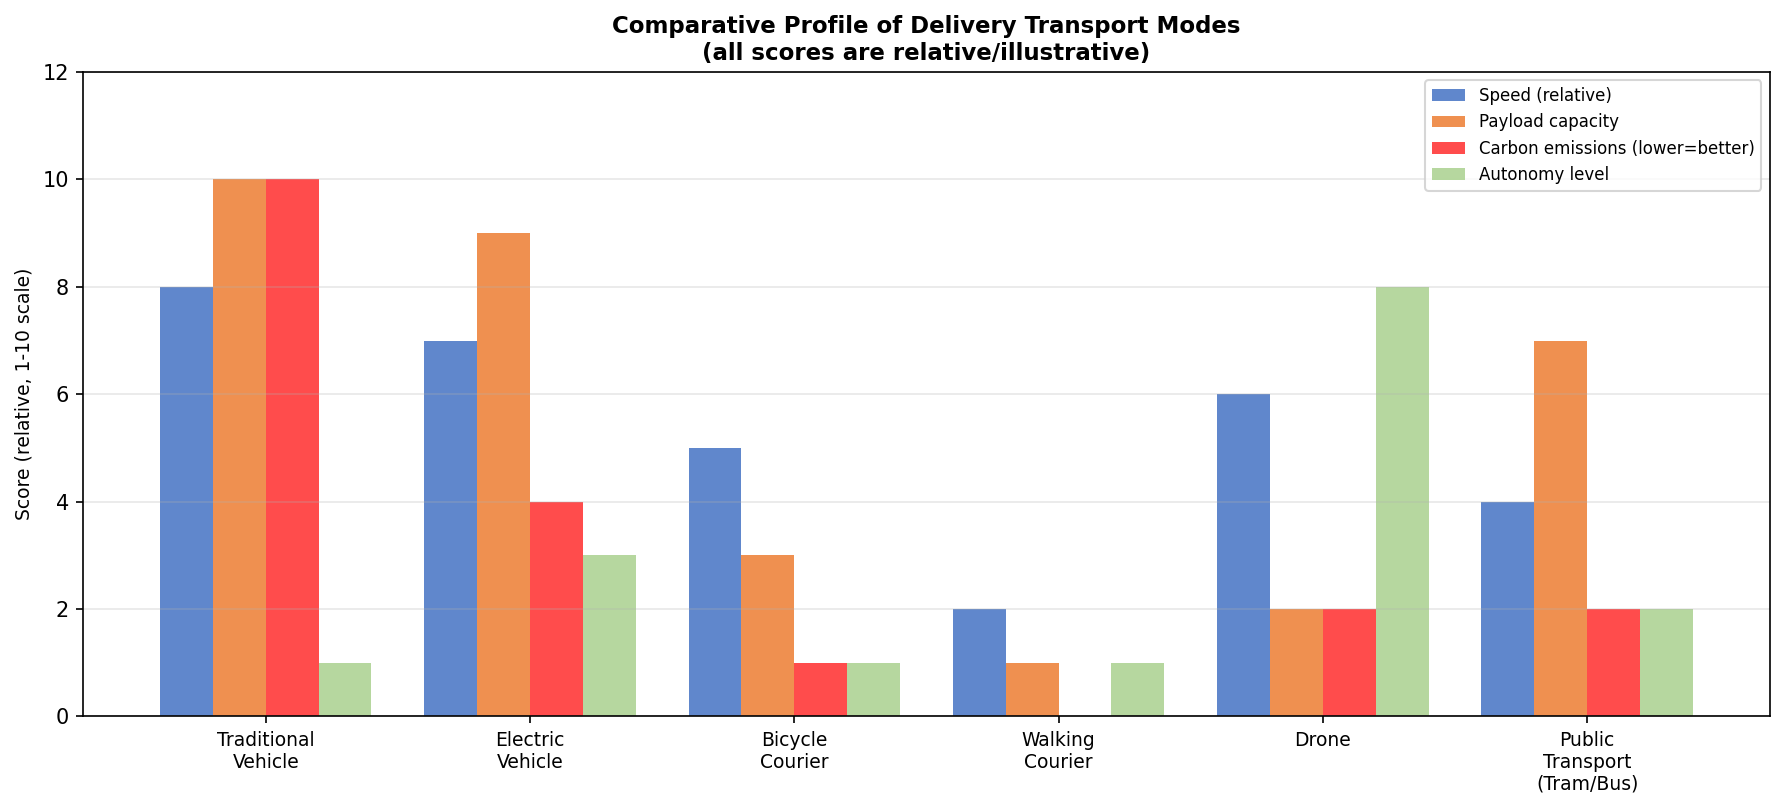
\includegraphics[width=0.90\textwidth]{transport_modes.png}
  \end{center}

  \bigskip
  \begin{block}{Four Major Technological Shifts}
    \begin{enumerate}
      \item \textbf{Autonomous vehicles} --- removing the human driver
            from the cost function.
      \item \textbf{Unmanned Aerial Vehicles (UAVs / drones)} ---
            accessing locations unreachable by road at very low cost
            per delivery.
      \item \textbf{Electric and alternative-fuel vehicles} ---
            changing the cost structure (energy vs.\ fuel) and
            range constraints of the fleet.
      \item \textbf{Public transport as freight carrier} ---
            using existing tram, bus, and rail networks to move
            parcels to urban micro-depots.
    \end{enumerate}
  \end{block}

\end{frame}

%% ---- Autonomous Vehicles ----
\begin{frame}[allowframebreaks]{13.2 Autonomous Vehicles}

  An autonomous vehicle (AV) is one that navigates and drives
  without a human operator.  The book notes that AVs offer
  two distinct advantages for delivery logistics:

  \bigskip
  \begin{block}{Advantages of Autonomous Delivery Vehicles}
    \begin{itemize}
      \item \textbf{Cost reduction.}
            The single largest cost in last-mile delivery is the
            \emph{driver's wage}.  An autonomous vehicle eliminates
            this cost entirely, potentially making small-load
            deliveries economically viable for the first time.

      \item \textbf{Flexibility.}
            An AV can operate 24 hours a day without fatigue
            regulations, enabling overnight or off-peak deliveries
            that reduce urban congestion during rush hours.
    \end{itemize}
  \end{block}

  \bigskip
  The book also highlights a key research challenge that emerges
  with AVs: \textbf{the multi-agent coordination problem}.  When
  many AVs from different companies operate in the same city,
  they must cooperate to avoid collisions, share charging
  infrastructure, and prevent the streets from becoming congested
  with empty-running vehicles.

  \bigskip
  \begin{exampleblock}{Worked Example: Multi-Agent Savings}
    Suppose two delivery companies each operate 10 AVs in the same
    city.  Without coordination, both fleets may converge on the
    same streets at the same time, doubling congestion and halving
    the effective road capacity.  With a shared routing protocol
    (e.g., a city-level swarm coordinator), the 20 AVs can be
    dispatched on non-overlapping routes, reducing total distance
    driven by an estimated 15--30\% (a figure consistent with
    cooperative VRP studies in the literature).
  \end{exampleblock}

  \bigskip
  \begin{alertblock}{Key Insight}
    The introduction of AVs does not simplify the optimisation
    problem --- it transforms it from a \emph{single-company}
    Vehicle Routing Problem into a \emph{multi-agent} coordination
    problem that may require city-level governance as well as
    algorithmic innovation.
  \end{alertblock}

\end{frame}

%% ---- Drones ----
\begin{frame}[allowframebreaks]{13.2 Drones and Unmanned Aerial Vehicles (UAVs)}

  Unmanned Aerial Vehicles (UAVs), commonly called drones, can fly
  directly from a depot or a truck to a customer's door, bypassing
  road congestion entirely.  The book cites multiple studies on
  drone-based delivery and identifies both the promise and the
  constraints:

  \bigskip
  \begin{block}{Why Drones Are Attractive for Last-Mile Delivery}
    \begin{itemize}
      \item \textbf{Speed.}
            A drone travels in a straight line (``as the crow flies''),
            avoiding road distance that can be 40--60\% longer than
            the geodesic distance in urban grids.

      \item \textbf{Access.}
            Rural or island locations that are expensive to serve
            by road can be reached at low marginal cost.
            The book cites drone delivery in the Pacific Islands and
            healthcare supply to remote clinics as real-world examples.

      \item \textbf{Low carbon footprint per delivery.}
            An electric drone carrying a small parcel produces far
            less CO\textsubscript{2} per delivery than a conventional
            van on a half-empty route.
    \end{itemize}
  \end{block}

  \bigskip
  \begin{block}{Constraints and Research Challenges}
    \begin{itemize}
      \item \textbf{Payload limit.}
            Current commercial drones carry at most 2--5 kg,
            which covers roughly 80\% of e-commerce parcels
            but excludes bulky items.

      \item \textbf{Range and battery.}
            Most delivery drones have an operational range of
            10--20 km per charge.  This means they must be
            recharged or replaced frequently, and the placement
            of charging stations becomes an important optimisation
            sub-problem.

      \item \textbf{Regulation.}
            Most national aviation authorities require drones to
            remain within visual line of sight (VLOS), which limits
            autonomous long-range operation.  The book notes that
            regulation is evolving rapidly.

      \item \textbf{Weather sensitivity.}
            Strong winds, rain, and fog can ground drone fleets,
            introducing uncertainty that must be handled by the
            routing algorithm.

      \item \textbf{Multi-organisation coordination.}
            When multiple companies operate drone fleets over the
            same city, a swarm-intelligence layer is needed to
            prevent mid-air collisions and to allocate airspace
            fairly.
    \end{itemize}
  \end{block}

  \bigskip
  \begin{center}
    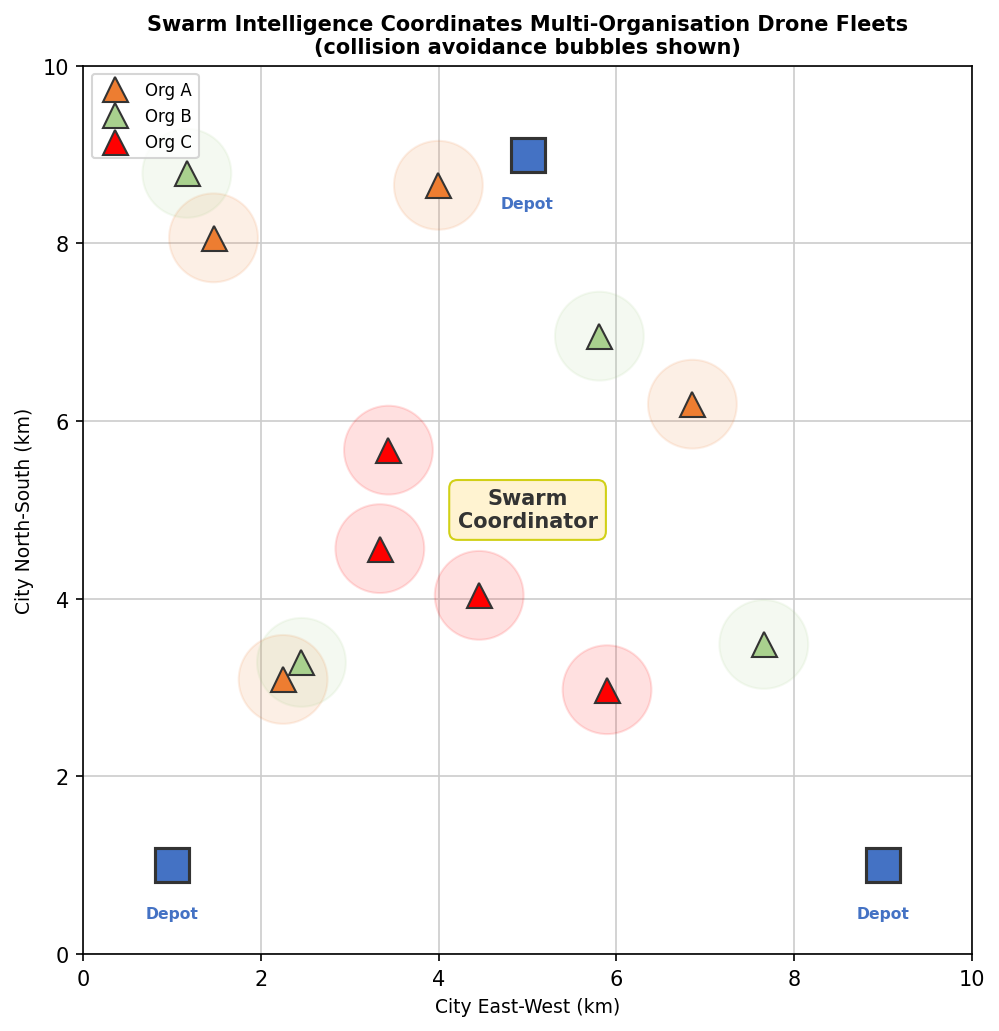
\includegraphics[width=0.72\textwidth]{drone_swarm.png}
  \end{center}

  \begin{alertblock}{Key Insight}
    The combination of a truck (for long-haul transport) and a drone
    (for the last few kilometres) --- the so-called
    \textbf{truck-and-drone problem} --- is one of the most
    actively studied variants of the VRP today.  It is inherently
    multi-objective: minimising time favours the drone, minimising
    energy cost may favour the truck, and minimising carbon
    emissions introduces a third trade-off axis.
  \end{alertblock}

\end{frame}

%% ---- Electric Vehicles ----
\begin{frame}[allowframebreaks]{13.2 Electric and Alternative-Fuel Vehicles}

  Electric vehicles (EVs) are already being adopted by major parcel
  carriers in Europe and North America.  Their impact on routing
  optimisation is not just environmental --- it changes the
  \emph{mathematical structure} of the problem.

  \bigskip
  \begin{block}{How EVs Change the VRP}
    A conventional vehicle routing problem assumes that a vehicle
    can travel any distance as long as it does not exceed its
    \emph{load capacity}.  An electric vehicle adds a second
    constraint: the \emph{state of charge} (SoC), which decreases
    with distance and increases only when the vehicle visits a
    charging station.  This gives rise to the
    \textbf{Electric Vehicle Routing Problem (E-VRP)}, which has
    the following additional features:

    \medskip
    \begin{itemize}
      \item \textbf{Charging station placement.}
            The locations of charging stations must be known in
            advance, and routes must be designed to visit them
            before the battery runs empty.

      \item \textbf{Non-linear charging time.}
            Batteries charge quickly when nearly empty but slowly
            when nearly full (the standard lithium-ion charge curve).
            This means a full recharge is rarely optimal: partial
            recharges at multiple stops may minimise total route time.

      \item \textbf{Range anxiety.}
            Even with careful planning, unexpected traffic or
            detours can drain the battery unexpectedly.
            Robust routing algorithms must plan with a safety margin.
    \end{itemize}
  \end{block}

  \bigskip
  \begin{exampleblock}{Worked Example: Range Constraint in a Route}
    Suppose an EV has a range of 120 km on a full charge and must
    serve five customers at distances (from depot) of 15, 30, 55,
    85, and 110 km.  A naive nearest-neighbour route visits them
    in order: $0 \to 15 \to 30 \to 55 \to 85 \to 110 \to 0$ km,
    for a total of approximately 140 km --- \emph{exceeding} the
    120 km range.  The vehicle would run out of charge before
    returning to the depot.  A good E-VRP solver would insert a
    stop at a charging station located, say, at km 70, adding
    perhaps 20 minutes of charging time but ensuring the route
    is feasible.  The trade-off between route length and
    charging stops is the core optimisation challenge.
  \end{exampleblock}

  \bigskip
  The book also notes that alternative fuels --- hydrogen, compressed
  natural gas, and hybrid propulsion --- are entering the fleet mix,
  each with different range, refuelling infrastructure, and
  environmental profiles.  Future solvers must be able to handle
  \emph{heterogeneous} fleets containing vehicles with different
  fuel types simultaneously.

\end{frame}

%% ---- Public Transport ----
\begin{frame}[allowframebreaks]{13.2 Public Transport as a Freight Carrier}

  An innovative idea gaining traction in European cities is to use
  \textbf{existing public transport networks} --- trams, buses,
  underground trains --- to carry parcels alongside passengers.

  \bigskip
  The concept addresses a fundamental problem in urban logistics:
  delivery vans travelling through city centres cause congestion
  and pollution precisely at the times and places where pedestrians
  and cyclists are most present.  If parcels could instead travel
  on trams that are already running, the number of delivery vans
  in the city centre could be reduced dramatically.

  \bigskip
  \begin{block}{How a Tram-Based Delivery Network Works}
    \begin{enumerate}
      \item Parcels from an out-of-town distribution centre are
            loaded onto a specially designed cargo tram (or into
            reserved space on a regular tram) at a \emph{city-edge
            terminal}.
      \item The tram carries the parcels along its scheduled route
            to \emph{micro-depots} located at tram stops.
      \item At each micro-depot, couriers on bicycles or on foot
            complete the \emph{last-mile delivery} to individual
            addresses within a few hundred metres of the stop.
    \end{enumerate}
  \end{block}

  \bigskip
  \begin{center}
    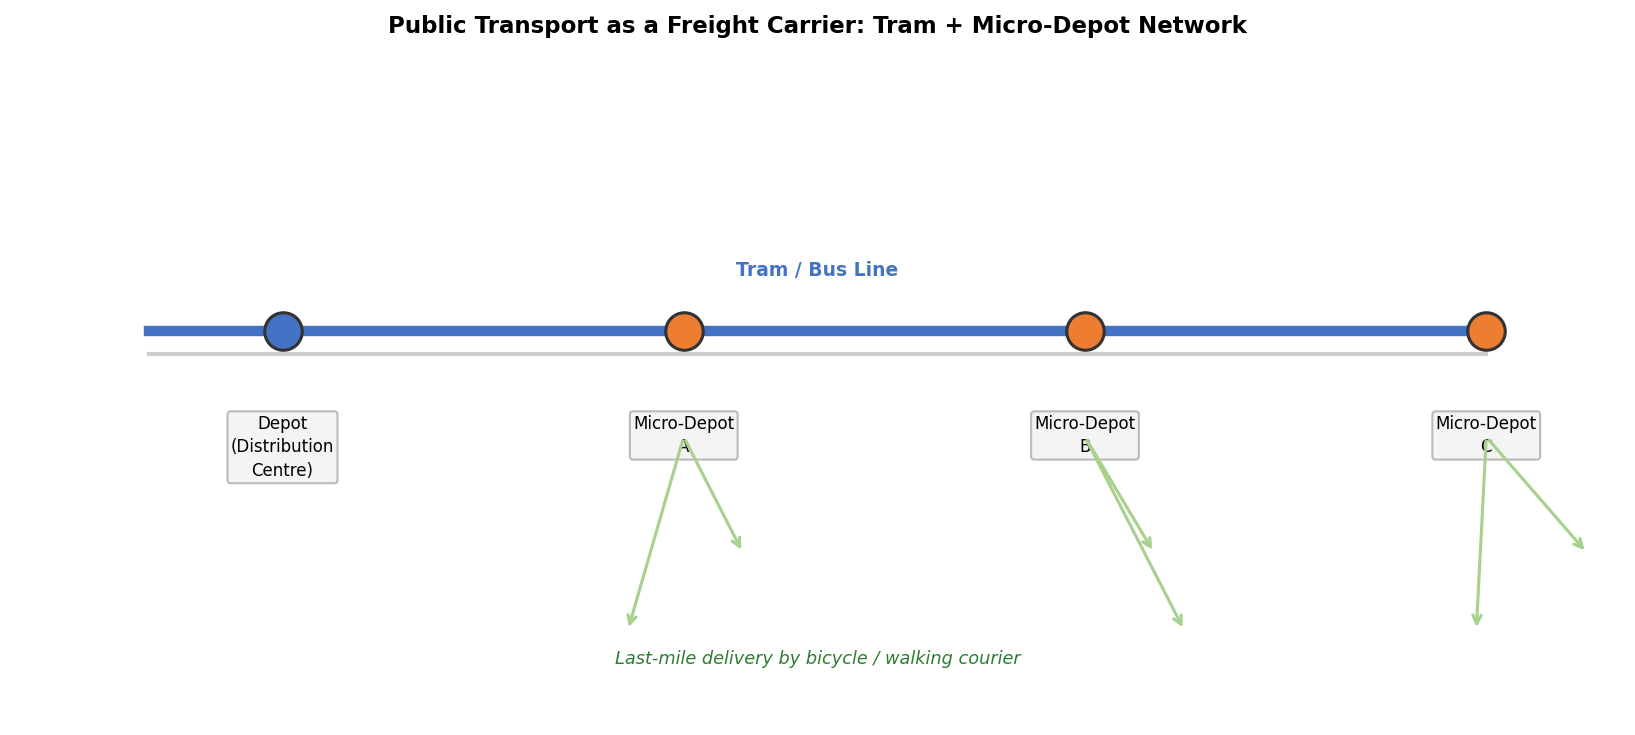
\includegraphics[width=0.88\textwidth]{public_transport.png}
  \end{center}

  \bigskip
  The book cites a study on cargo trams in Poland (Pietrzak and
  Pietrzak, 2021) as an example of this approach being tested in
  practice.  The optimisation challenge is to schedule which parcels
  travel on which tram service, determine micro-depot locations, and
  plan the last-mile courier routes --- all simultaneously.  This is
  a complex multi-modal routing problem that the metaheuristics
  covered earlier in the book are well suited to tackle.

  \begin{alertblock}{Key Insight}
    Public transport integration does not replace van delivery;
    it \emph{concentrates} van activity on routes between the
    distribution centre and the city edge, while replacing the
    more polluting urban leg with a zero-marginal-emission
    tram service.  The overall system becomes a two-tier
    logistics network, and optimising both tiers simultaneously
    is a rich research problem.
  \end{alertblock}

\end{frame}

%% ---- Python: E-VRP Range Check ----
\begin{frame}[fragile]{Python: Electric Vehicle Range Feasibility Check}

  The following Python function illustrates how to check whether
  a proposed route is feasible for an electric vehicle given its
  battery capacity and the distances between stops.  If the
  cumulative distance exceeds the range, the function identifies
  where the vehicle would need to stop for a recharge.

  \smallskip
  \begin{lstlisting}
def check_ev_feasibility(route, distance_matrix, ev_range_km,
                         charging_stations):
    """
    Checks whether a route is feasible for an electric vehicle.

    Parameters
    ----------
    route            : list of node indices, e.g. [0, 3, 7, 2, 0]
                       where 0 is the depot
    distance_matrix  : 2-D list / numpy array;
                       distance_matrix[i][j] = distance in km
    ev_range_km      : float, maximum range on a full charge
    charging_stations: set of node indices that are charging stations

    Returns
    -------
    dict with keys:
      'feasible'         : bool
      'charge_at'        : list of nodes where charging is needed
      'distance_segments': list of cumulative distances between charges
    """
    charge_at     = []
    segments      = []
    current_dist  = 0.0   # distance since last charge

    for i in range(len(route) - 1):
        node_from  = route[i]
        node_to    = route[i + 1]
        leg_dist   = distance_matrix[node_from][node_to]

        # Check: would adding this leg exhaust the battery?
        if current_dist + leg_dist > ev_range_km:
            # Must charge somewhere before node_to
            # Find nearest charging station on the path
            nearest_cs = find_nearest_charging_station(
                node_from, charging_stations, distance_matrix,
                ev_range_km - current_dist   # remaining range
            )
            if nearest_cs is None:
                # No reachable charging station -- route is infeasible
                return {'feasible': False,
                        'charge_at': charge_at,
                        'distance_segments': segments}
            charge_at.append(nearest_cs)
            segments.append(current_dist)
            current_dist = distance_matrix[nearest_cs][node_to]
        else:
            current_dist += leg_dist

    segments.append(current_dist)
    return {'feasible': True,
            'charge_at': charge_at,
            'distance_segments': segments}


def find_nearest_charging_station(current_node, stations,
                                  dist_matrix, remaining_range):
    """
    Returns the nearest reachable charging station from current_node,
    or None if no station is within remaining_range.
    """
    reachable = [s for s in stations
                 if dist_matrix[current_node][s] <= remaining_range]
    if not reachable:
        return None
    return min(reachable, key=lambda s: dist_matrix[current_node][s])
  \end{lstlisting}

  \smallskip
  \textbf{How the code works:}
  The function walks along the route step by step.  The variable
  \texttt{current\_dist} tracks the distance driven since the last
  charge (initialised to zero at the depot).  At each step, it checks
  whether adding the next leg would push the total beyond
  \texttt{ev\_range\_km} (the vehicle's maximum range).  If so, it
  searches for a reachable charging station, inserts a charging stop,
  resets the distance counter, and continues.  If no charging station
  is reachable, the route is declared infeasible.

\end{frame}

%% ====================================================================
\section{13.3 Consumers}
%% ====================================================================

\begin{frame}[allowframebreaks]{13.3 Consumers --- The Demand Side}

  Technology on the supply side (better algorithms, autonomous
  vehicles, drones) is only one half of the picture.  The other
  half is the \emph{demand side}: what consumers expect from
  delivery services, and how those expectations are changing.

  \bigskip
  \begin{center}
    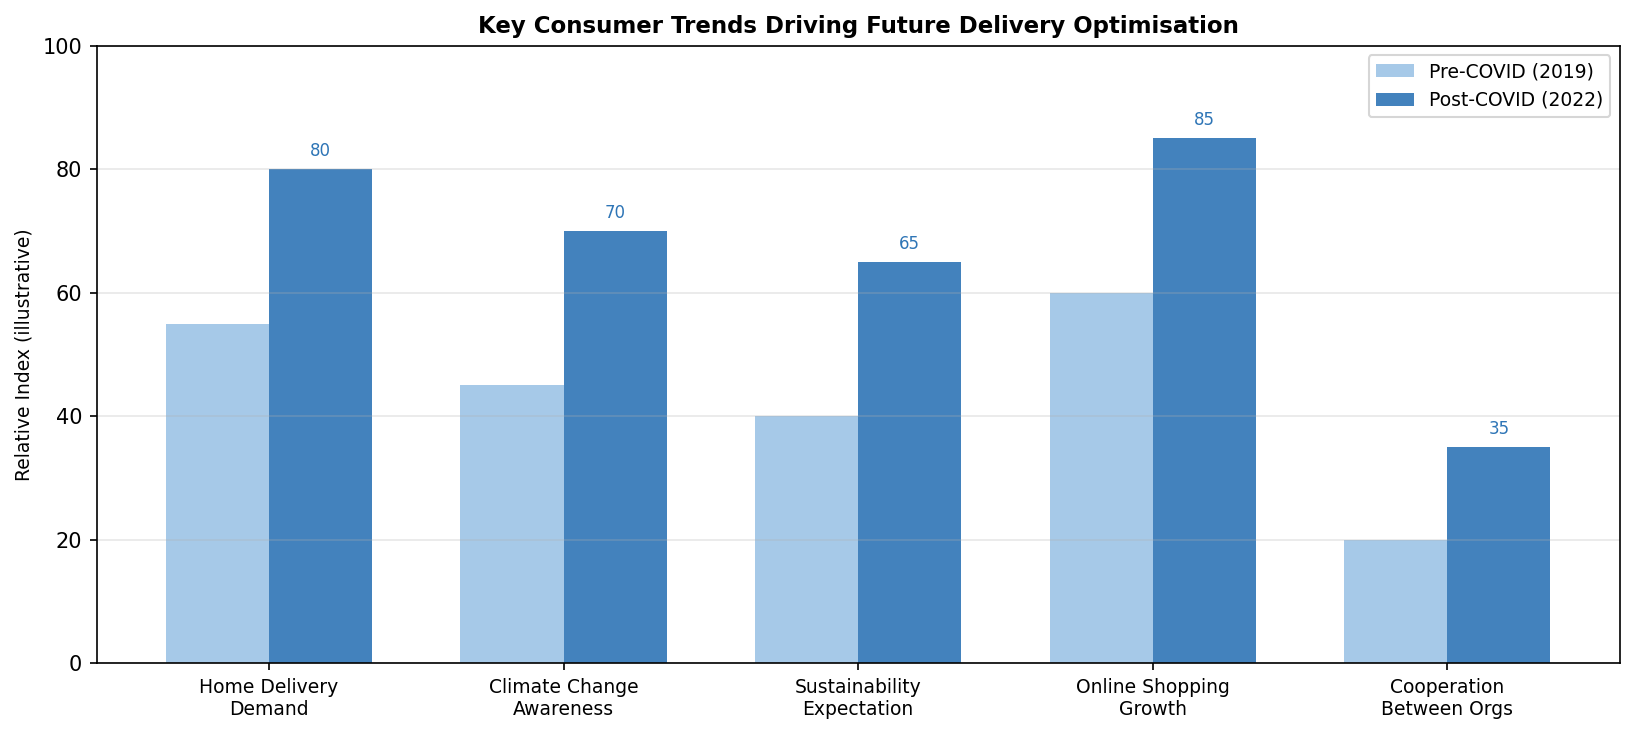
\includegraphics[width=0.88\textwidth]{consumer_trends.png}
  \end{center}

  \bigskip
  \begin{block}{Three Overarching Trends Identified in the Book}
    \begin{enumerate}
      \item \textbf{Increasing demand for home delivery.}
            The COVID-19 pandemic dramatically accelerated the
            long-running shift from in-store shopping to
            e-commerce.  Home delivery volumes approximately
            doubled in many markets between 2019 and 2021,
            and this growth is expected to persist.

      \item \textbf{Growing awareness of climate change.}
            Consumers are increasingly aware that every delivery
            has a carbon footprint, and a growing minority
            is willing to pay a premium for greener delivery
            options (e.g., consolidated next-day delivery
            rather than same-day).

      \item \textbf{Pressure for sustainability from multiple directions.}
            Climate-change awareness is pushing both consumers
            and regulators to demand lower-emission delivery
            systems, creating a strong incentive for carriers
            to invest in electric fleets, route optimisation,
            and consolidation.
    \end{enumerate}
  \end{block}

\end{frame}

%% ---- Failed Deliveries ----
\begin{frame}[allowframebreaks]{13.3 The Problem of Failed Deliveries}

  One of the most costly and environmentally damaging outcomes in
  last-mile logistics is a \textbf{failed delivery}: the vehicle
  arrives at a customer address but nobody is home to accept the
  parcel.  The book discusses this in detail because it illustrates
  the tight coupling between consumer behaviour and optimisation.

  \bigskip
  \begin{block}{Why Failed Deliveries Are Expensive}
    \begin{itemize}
      \item \textbf{Direct cost.}
            The vehicle has consumed fuel and driver time
            (or in the EV case, battery charge) without completing
            a delivery.  The parcel must be returned to a depot
            and either re-delivered or collected.

      \item \textbf{Environmental cost.}
            The failed delivery represents ``wasted'' vehicle
            kilometres that produce CO\textsubscript{2} with no
            useful outcome.

      \item \textbf{Knock-on effect.}
            Returning to re-deliver disrupts the planned route
            for subsequent stops, potentially causing cascading
            late deliveries.
    \end{itemize}
  \end{block}

  \bigskip
  \begin{exampleblock}{Worked Example: Cost of a 10\% Failure Rate}
    Consider a depot that dispatches 100 vehicles, each serving
    50 customers per day.  If the failed-delivery rate is 10\%,
    then on average each vehicle fails to deliver at 5 stops.
    If re-delivery requires a dedicated return trip of 3 km
    per failed stop, and the vehicle emits 200 g CO\textsubscript{2}
    per km, then:

    \[
      \text{Wasted distance per vehicle} = 5 \times 3 = 15 \text{ km}
    \]
    \[
      \text{Extra emissions per vehicle} = 15 \times 200 = 3{,}000 \text{ g}
      = 3 \text{ kg CO}_2
    \]
    \[
      \text{Fleet-wide extra emissions} = 100 \times 3 = 300 \text{ kg CO}_2
      \text{ per day}
    \]

    Over a year (250 working days) this amounts to
    $300 \times 250 = 75{,}000$ kg = 75 tonnes of avoidable CO\textsubscript{2}.
    For a medium-sized carrier, this is a significant fraction of
    the fleet's total carbon footprint.
  \end{exampleblock}

  \bigskip
  \begin{alertblock}{Key Insight}
    Reducing the failed-delivery rate is not just a customer-service
    problem; it is an environmental and economic one.  Approaches
    include better delivery-window estimation, smart parcel lockers,
    and dynamic re-routing that responds to real-time customer
    availability data.
  \end{alertblock}

\end{frame}

%% ---- Cooperative Delivery ----
\begin{frame}[allowframebreaks]{13.3 Cooperation Between Organisations}

  A theme that runs throughout the book's conclusions is that
  many of the hardest challenges in delivery logistics cannot
  be solved by any single organisation acting alone.
  \textbf{Cross-organisational cooperation} offers significant
  efficiency gains, but requires trust, data sharing, and
  potentially new regulatory frameworks.

  \bigskip
  \begin{center}
    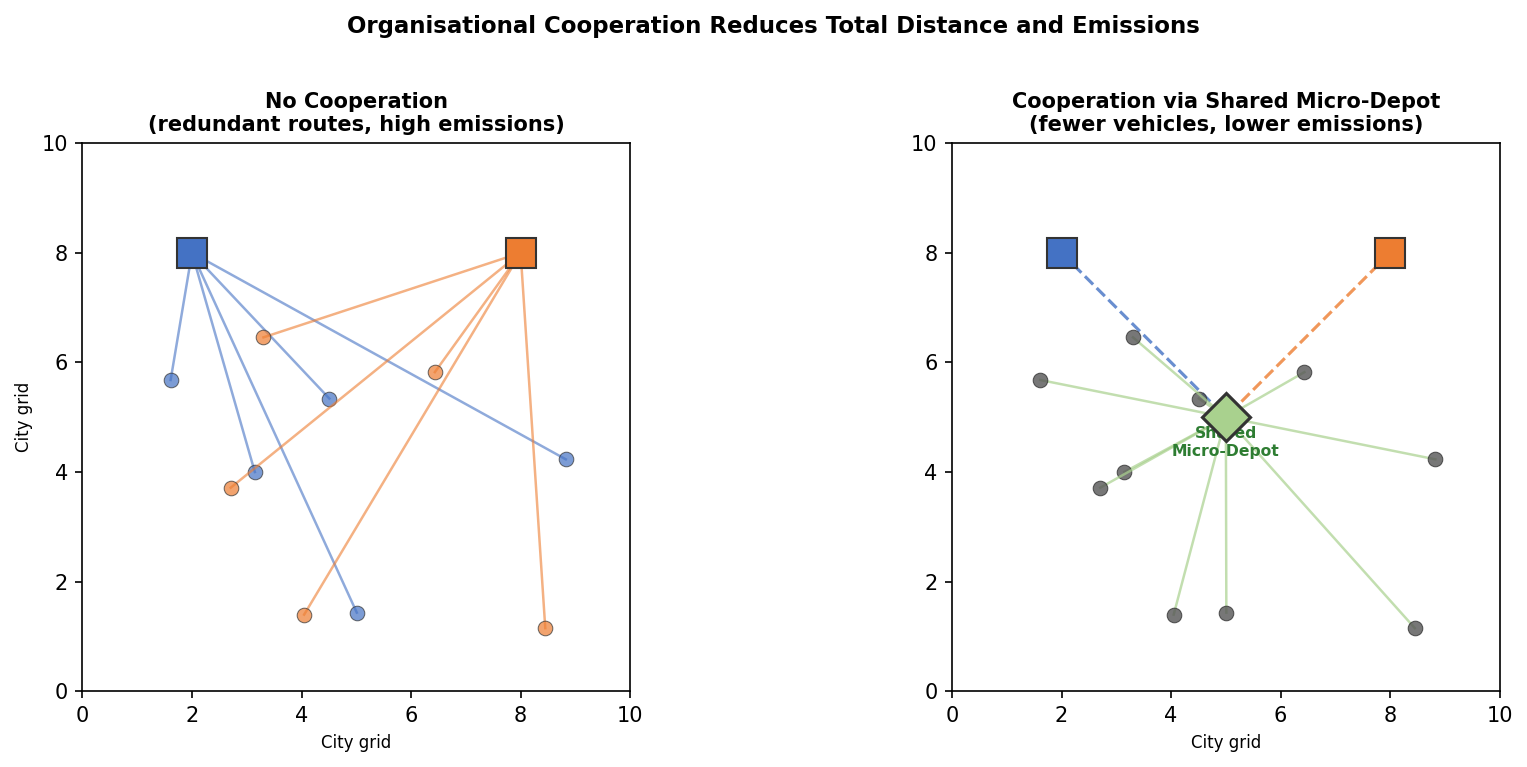
\includegraphics[width=0.88\textwidth]{cooperation.png}
  \end{center}

  \bigskip
  \begin{block}{Forms of Cooperative Delivery}
    \begin{itemize}
      \item \textbf{Shared micro-depots.}
            Two or more companies share a city-centre mini-warehouse.
            Parcels from different carriers are consolidated
            and delivered together by a single courier, halving
            the number of vehicles in the area.

      \item \textbf{Route sharing.}
            Carriers compare planned routes and identify overlapping
            segments.  Where two vehicles are heading in the same
            direction, one can carry the other's parcels for part
            of the journey (analogous to ridesharing for freight).

      \item \textbf{Drone swarms across organisations.}
            Multiple companies' drone fleets share a city-level
            airspace management system that ensures collision
            avoidance and fair allocation of flight paths.
    \end{itemize}
  \end{block}

  \bigskip
  \begin{exampleblock}{Worked Example: Savings from Cooperation}
    Studies cited in the book suggest that route-sharing between
    two medium-sized carriers typically reduces total distance
    driven by \textbf{15--25\%} without increasing delivery times.
    For a combined fleet of 200 vehicles each driving 100 km/day,
    this amounts to:
    \[
      \text{Distance saving} = 200 \times 100 \times 0.20 = 4{,}000 \text{ km/day}
    \]
    At 200 g CO\textsubscript{2}/km, this is 800 kg = 0.8 tonnes of
    CO\textsubscript{2} saved \emph{every single day}.
  \end{exampleblock}

  \bigskip
  \begin{alertblock}{Key Insight}
    Cooperation transforms the optimisation problem from a
    single-company VRP into a \emph{collaborative VRP} (ColVRP),
    where the objective function includes a fairness term
    to ensure each partner benefits.  This is an active and
    largely unsolved research area.
  \end{alertblock}

\end{frame}

%% ---- Sustainability ----
\begin{frame}[allowframebreaks]{13.3 Sustainability as a Design Constraint}

  The book argues that sustainability --- reducing carbon emissions,
  minimising wasted trips, and using vehicles efficiently --- is
  no longer an optional add-on but a core design constraint for
  future delivery systems.

  \bigskip
  Consumer pressure, regulation (e.g., low-emission zones in
  European cities), and corporate net-zero commitments are all
  converging to make \emph{green routing} the default mode of
  operation for forward-looking carriers.

  \bigskip
  \begin{block}{Sustainability Levers Available to Carriers}
    \begin{description}
      \item[Fleet electrification.]
            Replacing diesel vans with EVs eliminates tailpipe
            emissions at the point of delivery.  When charged on
            renewable energy, the lifecycle emissions approach zero.

      \item[Parcel consolidation.]
            Combining multiple small orders into a single larger
            delivery (perhaps with a one-day delay) reduces the
            total number of vehicle trips.  The book notes that
            even modest consolidation rates of 20--30\% can
            cut vehicle-kilometres by 10--15\%.

      \item[Green routing.]
            Route optimisation algorithms can be extended to
            minimise fuel consumption or CO\textsubscript{2} rather
            than simply minimising distance or time.
            Because fuel consumption depends on speed, gradient,
            and load --- not just distance --- this requires more
            detailed vehicle models but is achievable with the
            techniques covered in this book.

      \item[Consumer-side interventions.]
            Offering financial incentives for flexible delivery
            windows, consolidated deliveries, or parcel-locker
            collection can shift consumer behaviour in ways that
            make routing more efficient.
    \end{description}
  \end{block}

  \bigskip
  \begin{alertblock}{Key Insight}
    The most powerful sustainability interventions often act on
    multiple levers simultaneously.  For example, a carrier that
    electrifies its fleet \emph{and} consolidates parcels \emph{and}
    uses green routing can achieve far greater emissions reductions
    than any single measure alone.  Multi-objective optimisation ---
    a central theme of this book --- is the natural mathematical
    framework for managing these trade-offs.
  \end{alertblock}

\end{frame}

%% ====================================================================
\section{Book Summary and Conclusion}
%% ====================================================================

\begin{frame}[allowframebreaks]{Book Summary: Thirteen Chapters in Perspective}

  This concluding slide situates the chapter's forward-looking
  discussion within the broader arc of the book.

  \bigskip
  \begin{center}
    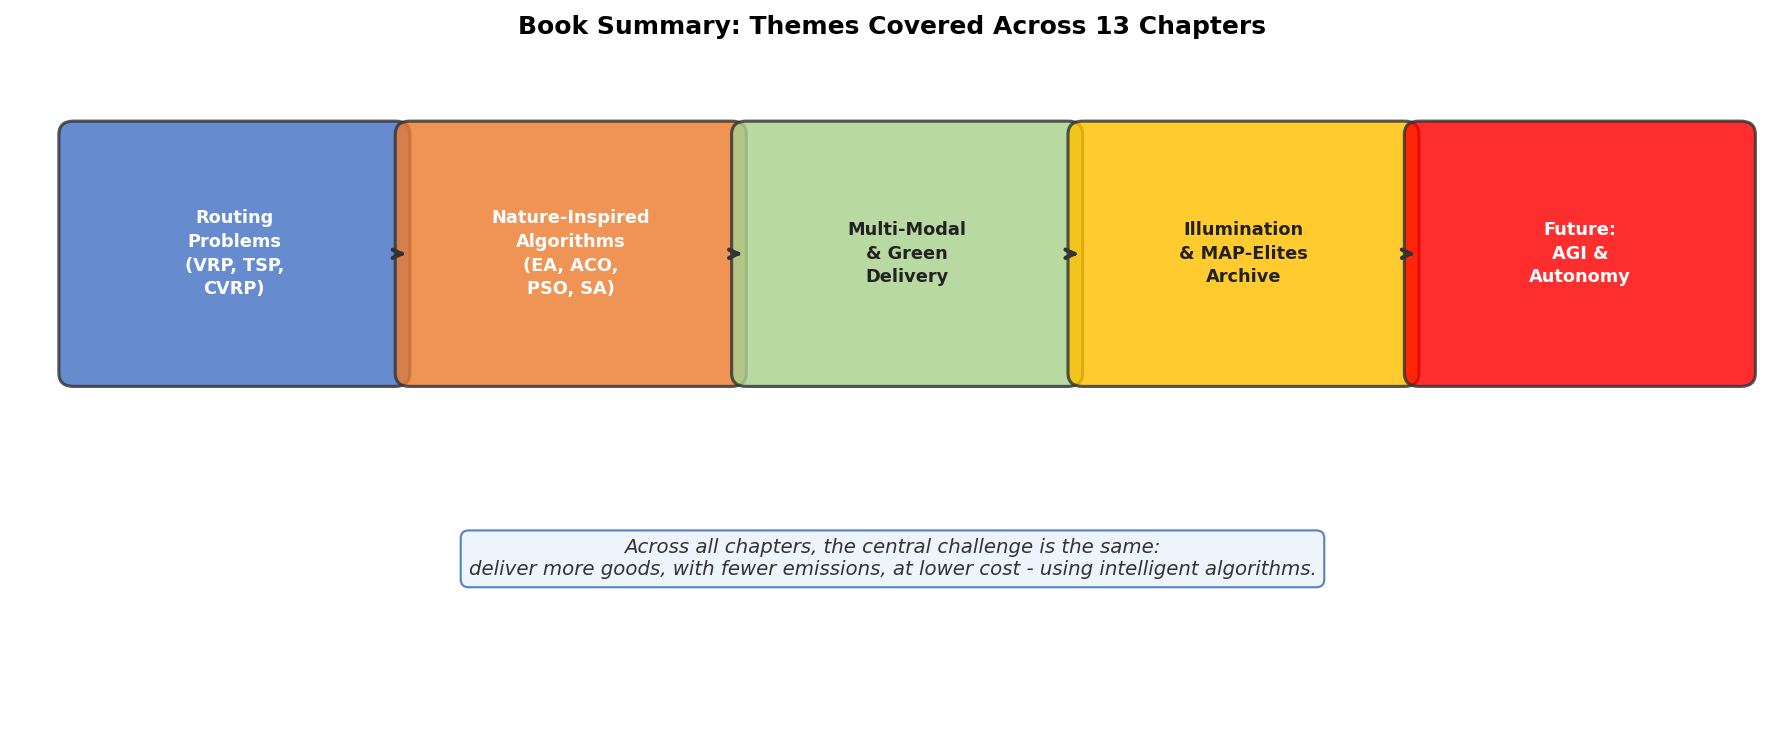
\includegraphics[width=0.90\textwidth]{book_summary.png}
  \end{center}

  \bigskip
  \begin{block}{What the Book Has Shown}
    \begin{itemize}
      \item \textbf{Chapters 1--4} established the fundamental
            routing problems (TSP, VRP, CVRP) and the first-generation
            nature-inspired algorithms (evolutionary computation,
            local search) that solve them.

      \item \textbf{Chapters 5--6} extended the single-objective
            framework to multi-objective problems and introduced the
            illumination paradigm (MAP-Elites), which produces
            a diverse archive of high-quality solutions rather than
            a single ``best'' answer.

      \item \textbf{Chapters 7--9} showed how to incorporate
            real-world data --- geospatial information, traffic
            patterns, operational constraints --- into the
            optimisation models, bridging the gap between
            academic benchmarks and practical deployment.

      \item \textbf{Chapters 10--12} applied these techniques to
            three concrete industries: food delivery, letter
            (postal) delivery, and parcel delivery.  Each case
            study revealed industry-specific constraints and
            performance benchmarks.

      \item \textbf{Chapter 13} (this chapter) looks ahead to the
            algorithmic, technological, and societal changes
            that will define the next decade of delivery logistics.
    \end{itemize}
  \end{block}

\end{frame}

%% ---- Final Conclusions ----
\begin{frame}[allowframebreaks]{Final Conclusions}

  The book ends with a statement that captures the authors'
  central conviction:

  \bigskip
  \begin{block}{Central Message}
    \textit{``The field of delivery optimisation stands at a moment
    of profound change.  The algorithms developed over the past three
    decades --- genetic algorithms, ant colony optimisation, simulated
    annealing, MAP-Elites --- provide a solid mathematical foundation.
    But the problems ahead are harder, the systems are more complex,
    and the stakes are higher: climate change, urban congestion, and
    the expectations of billions of online shoppers are all converging
    on the logistics industry at the same time.''}
  \end{block}

  \bigskip
  \begin{columns}[t]
    \column{0.48\textwidth}
    \begin{block}{What the Next Generation of Solvers Must Do}
      \begin{itemize}
        \item Handle heterogeneous, multi-modal fleets
              (vans, EVs, drones, trams) in a single model.
        \item Operate in real time as conditions change
              (dynamic VRP).
        \item Incorporate sustainability objectives
              as first-class constraints, not afterthoughts.
        \item Learn from past experience to avoid
              re-solving problems from scratch.
        \item Coordinate across organisations,
              not just within a single company's fleet.
      \end{itemize}
    \end{block}

    \column{0.48\textwidth}
    \begin{block}{What This Book Provides}
      \begin{itemize}
        \item A rigorous introduction to the mathematical
              structure of routing problems.
        \item A toolkit of nature-inspired algorithms
              that are both effective and adaptable.
        \item A framework (illumination / MAP-Elites)
              for exploring the trade-off space of
              multi-objective problems.
        \item Real-world case studies that show how
              to move from algorithm to deployment.
        \item A research agenda pointing toward the
              open problems that remain unsolved.
      \end{itemize}
    \end{block}
  \end{columns}

  \bigskip
  \begin{alertblock}{Final Thought}
    Nature-inspired optimisation --- algorithms that borrow
    the principles of evolution, ant foraging, and particle
    swarms --- has proven to be remarkably well suited to the
    complex, noisy, constraint-rich problems of real-world
    delivery logistics.  The challenge for the coming decade
    is to build these algorithms into intelligent, adaptive,
    sustainable systems that serve both the economy and the
    planet.
  \end{alertblock}

\end{frame}

%% ---- References ----
\begin{frame}[allowframebreaks]{References}

  The following works are cited in Chapter 13 of the book.
  They provide starting points for further reading on the
  topics covered in this chapter.

  \bigskip
  \begin{small}
  \begin{itemize}
    \item Koshta, N., Devi, Y., and Patra, S. (2021).
          Aerial bots in the supply chain: A new ally to combat
          COVID-19. \textit{Technology in Society}, \textbf{66},
          101646.

    \item Kurzweil, R. (2005).
          \textit{The Singularity is Near: When Humans Transcend
          Biology}. New York: Viking.

    \item Moshref-Javadi, M. and Winkenbach, M. (2021).
          Applications and research avenues for drone-based
          models in logistics: A classification and review.
          \textit{Expert Systems with Applications}, \textbf{177},
          114854.

    \item Pietrzak, O. and Pietrzak, K. (2021).
          Cargo tram in freight handling in urban areas in Poland.
          \textit{Sustainable Cities and Society}, \textbf{70},
          102902.

    \item Spanaki, K., Karafili, E., Sivarajah, U., Despoudi, S.,
          and Irani, Z. (2021).
          Artificial intelligence and food security: Swarm
          intelligence of AgriTech drones for smart AgriFood
          operations.
          \textit{Production Planning \& Control}, 1--19.
  \end{itemize}
  \end{small}

\end{frame}

\end{document}
